\chapter{Wyniki testów}
\label{ch:tests}

\section{Obszerne testy aplikacji}
$TODO$ obszerne testy, porównanie metod: LRA*, WHCA* przy tych samych warunkach początkowych, porównanie czasu wykonania, porównanie tego samego algorytmu w zależności od parametru (np. okna czasowego); badanie skuteczności, długości tras, czasu wykonania, 
do przeprowadzenia testów wykorzystano biblitekę jUnit, która co prawda służy do wykonywania testów jednostkowych sprawdzających poprawność pojedynczych komponentów aplikacji
metodyka przeprowadzenia testów
3 typy środowisk testowych (rozmiar, roboty, screeny)
histogram liczby kroków potrzebnych do rozwiązania
potwierdzenie oczekiwań (poprawności) - nigdy nie było tak, żeby LRA był lepszy
zwykłego A* nawet nie warto testować
potential field - nawet nie warto testować, raczej jako ciekawostka, nie potrafi doprowadzić do celu nawet jednego robota
przeprowadzenie testów jest trudne i wymaga losowania środowisk i warunków i wyciągania statystyki

\section{Screeny}
$TODO$ screeny ciekawych przypadków

\begin{figure}
	\centering
	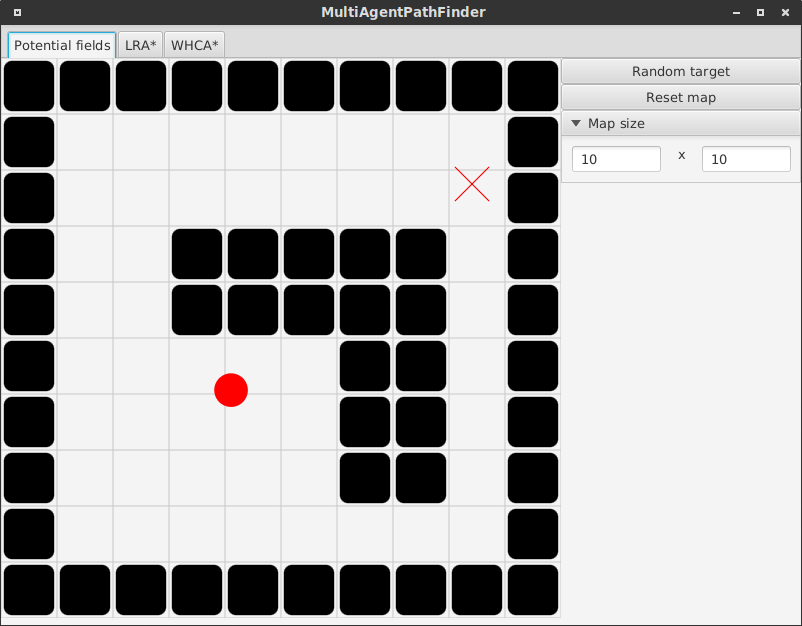
\includegraphics[width=0.8\columnwidth]{img/robopath/field-potential-hole}
	\caption{Robot uwięziony w studni potencjału. Zerowa siła wypadkowa nie pozwala mu dotrzeć do celu.}
	\label{fig:app-tech-intellij}
\end{figure}

\begin{figure}
	\centering
	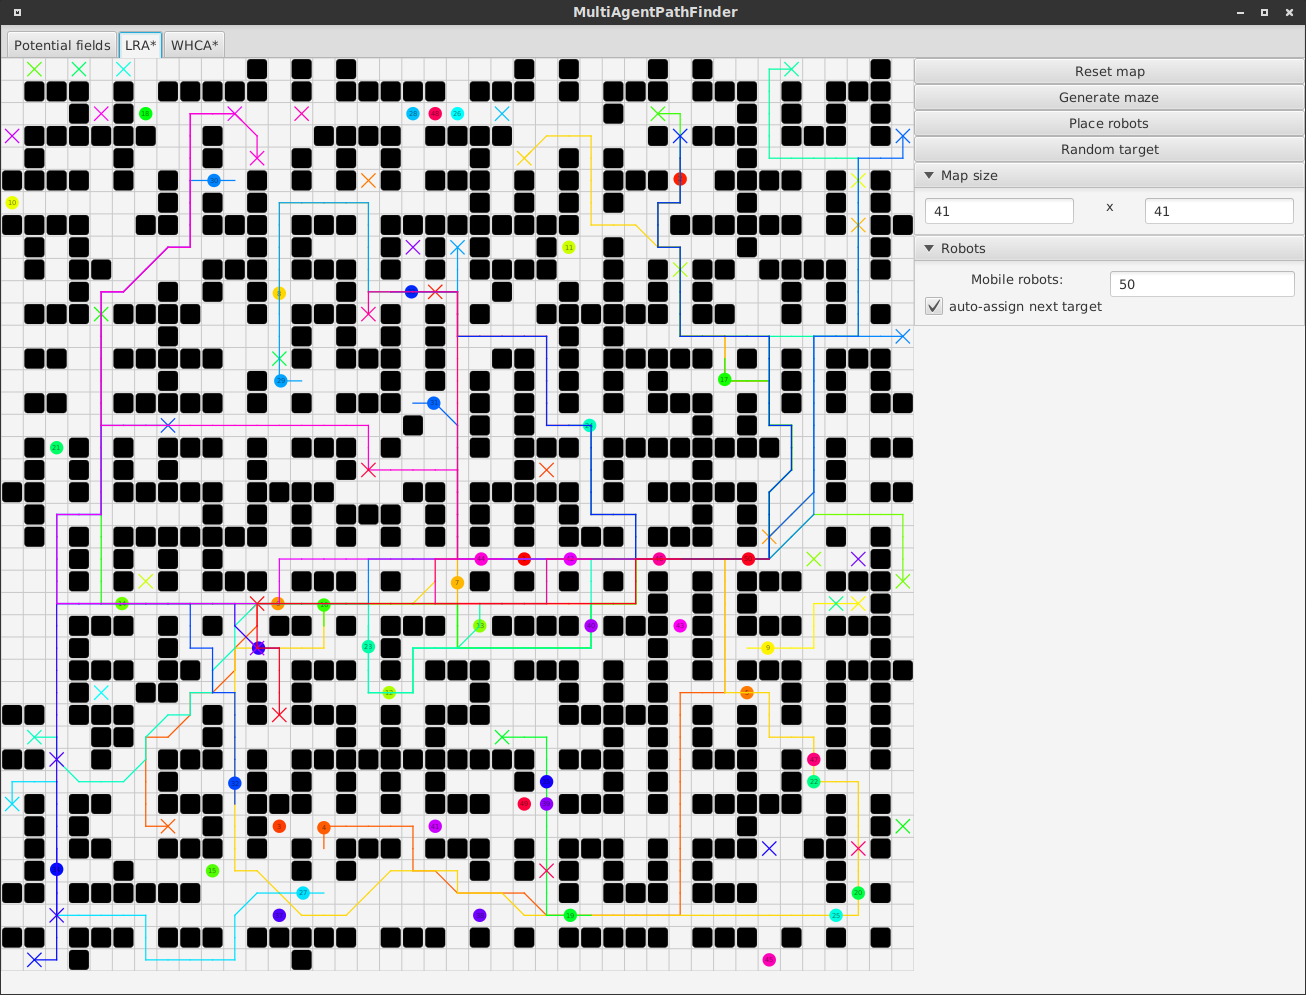
\includegraphics[width=0.8\columnwidth]{img/robopath/lra-bigmap}
	\caption{Metoda LRA*: duża mapa z dużą liczbą robotów}
	\label{fig:app-tech-intellij}
\end{figure}

\begin{figure}
	\centering
	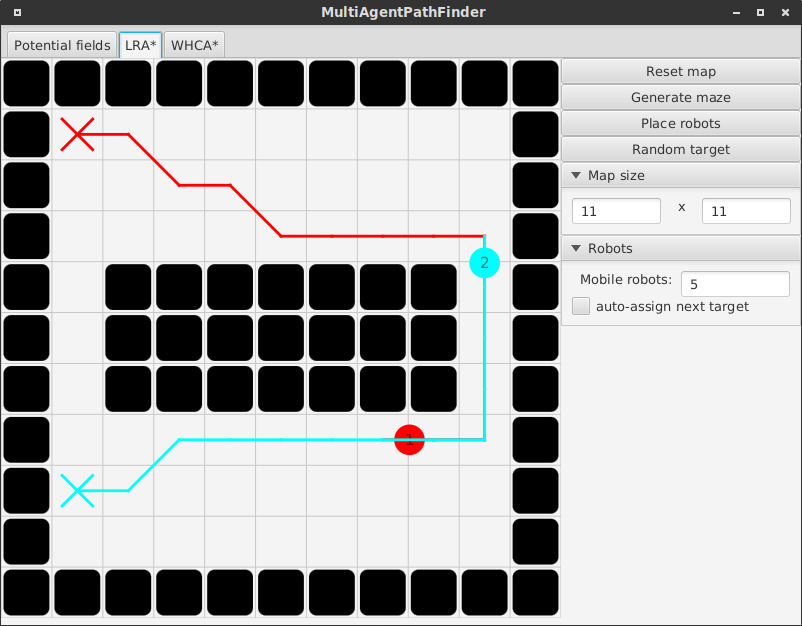
\includegraphics[width=0.8\columnwidth]{img/robopath/lra-cycle}
	\caption{Metoda LRA*: 2 roboty w cyklu akcji}
	\label{fig:app-tech-intellij}
\end{figure}

\begin{figure}
	\centering
	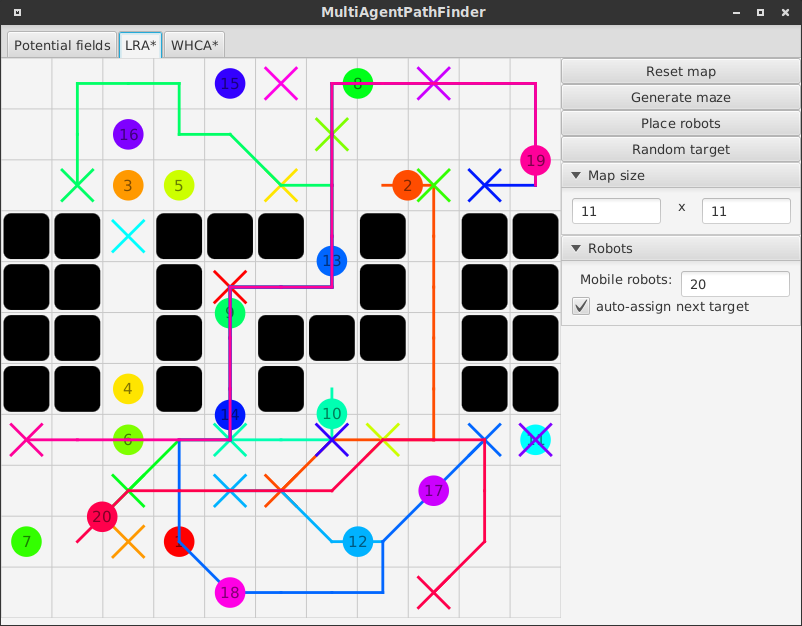
\includegraphics[width=0.8\columnwidth]{img/robopath/lra-lot-robots}
	\caption{Metoda LRA*: dużo robotów, mała mapa}
	\label{fig:app-tech-intellij}
\end{figure}

\begin{figure}
	\centering
	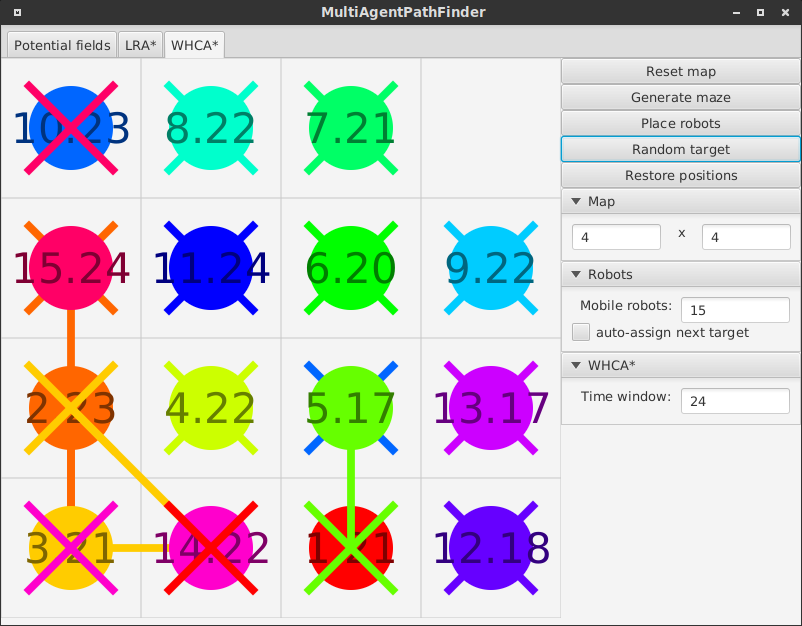
\includegraphics[width=0.8\columnwidth]{img/robopath/puzzle-15}
	\caption{Metoda WHCA*: puzzle 15}
	\label{fig:app-tech-intellij}
\end{figure}

\section{Środowiska}
labirynt, otwarte, puzzle 15

filmiki można obejrzć na YT, link

LRA: wyszło całkiem nieźle,
testy ograniczać trzeba liczbą kroków symulacji, bo LRA może trwać wiecznie

\section{Porównanie wyników}
jak często zwykły A* to za mało - ile razy pojawia się chociaż jedna kolizja?
porównanie WHCA* przy różnych oknach czasowych
porównanie metod przydziału i zmiany priorytetów - jak zmienia się skuteczność  po wprowadzeniu zmiany priorytetów
porównanie LRA* z WHCA*
porównanie CA* z WHCA*
porównanie z potential fields
porównanie WHCA z promocją priorytetów (własną, autorską) i bez + z/bez rozszerzania okna czasowego

\section{Dyskusja wyników}
wolno działa WHCA* przy dużych mapach / oknach czasu / robotach. Dałoby się zoptymalizować (RRA)
autorski WHCA* działa dobrze nawet przy rozwiązywaniu dużych deadlocków, problem z puzzle 15
